\documentclass[11pt,letterpaper]{article}
\usepackage[margin=0.6in]{geometry}
\usepackage{amsmath,amssymb}
\usepackage{tikz}
\usetikzlibrary{arrows.meta,positioning}
\usepackage{xcolor}
\usepackage{fontawesome5}
\usepackage{tcolorbox}
\usepackage{multicol}
\usepackage{enumitem}
\usepackage{hyperref}

\definecolor{primaryblue}{RGB}{41, 98, 255}
\definecolor{accentgreen}{RGB}{0, 150, 136}
\definecolor{warnorange}{RGB}{255, 152, 0}
\definecolor{lightgray}{RGB}{245, 245, 245}

\tcbset{
    conceptbox/.style={colback=primaryblue!5, colframe=primaryblue, boxrule=1pt, arc=3pt, left=5pt, right=5pt, top=5pt, bottom=5pt},
    formulabox/.style={colback=lightgray, colframe=gray!50, boxrule=0.5pt, arc=2pt, left=5pt, right=5pt, top=3pt, bottom=3pt},
    warningbox/.style={colback=warnorange!10, colframe=warnorange, boxrule=1pt, arc=3pt, left=5pt, right=5pt, top=5pt, bottom=5pt},
    appbox/.style={colback=accentgreen!5, colframe=accentgreen, boxrule=1pt, arc=3pt, left=5pt, right=5pt, top=5pt, bottom=5pt}
}

\pagestyle{empty}
\setlength{\parindent}{0pt}
\setlist[itemize]{leftmargin=*, itemsep=1pt, topsep=2pt}

\begin{document}

\begin{center}
{\LARGE\bfseries\color{primaryblue} Chapter 3: Calculus Foundations}\\[3pt]
{\large Gradients, Chain Rule, and Backpropagation}
\end{center}
\vspace{-5pt}
\hrule height 2pt
\vspace{8pt}

\begin{multicols}{2}

\begin{tcolorbox}[conceptbox, title={\faLightbulb\ Key Concepts}]
\begin{itemize}
    \item \textbf{Derivative}: Rate of change, slope of tangent
    \item \textbf{Partial Derivative}: Derivative w.r.t. one variable
    \item \textbf{Gradient}: Vector of all partial derivatives
    \item \textbf{Chain Rule}: Derivatives of composed functions
    \item \textbf{Jacobian}: Matrix of partial derivatives
    \item \textbf{Hessian}: Matrix of second derivatives
\end{itemize}
\end{tcolorbox}

\begin{tcolorbox}[formulabox, title={\faCalculator\ Core Formulas}]
\textbf{Gradient:}
\[ \nabla f = \left[ \frac{\partial f}{\partial x_1}, \ldots, \frac{\partial f}{\partial x_n} \right]^T \]

\textbf{Chain Rule (scalar):}
\[ \frac{d}{dx} f(g(x)) = f'(g(x)) \cdot g'(x) \]

\textbf{Chain Rule (vector):}
\[ \frac{\partial L}{\partial \mathbf{x}} = \frac{\partial L}{\partial \mathbf{y}} \cdot \frac{\partial \mathbf{y}}{\partial \mathbf{x}} \]

\textbf{Jacobian:}
\[ J_{ij} = \frac{\partial f_i}{\partial x_j} \]
\end{tcolorbox}

\columnbreak

\begin{center}
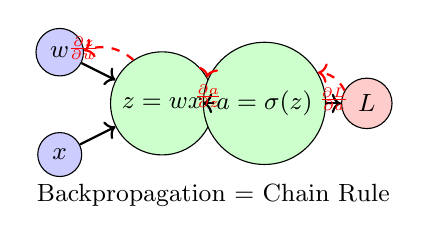
\begin{tikzpicture}[scale=0.65, every node/.style={font=\small}]
    % Computational graph
    \node[draw, circle, fill=blue!20] (x) at (0,0) {$x$};
    \node[draw, circle, fill=blue!20] (w) at (0,2) {$w$};
    \node[draw, circle, fill=green!20] (z) at (2,1) {$z=wx$};
    \node[draw, circle, fill=green!20] (a) at (4,1) {$a=\sigma(z)$};
    \node[draw, circle, fill=red!20] (L) at (6,1) {$L$};

    \draw[->,thick] (x) -- (z);
    \draw[->,thick] (w) -- (z);
    \draw[->,thick] (z) -- (a);
    \draw[->,thick] (a) -- (L);

    % Backward arrows
    \draw[->,red,dashed,thick] (L) to[bend right=30] node[below]{\tiny $\frac{\partial L}{\partial a}$} (a);
    \draw[->,red,dashed,thick] (a) to[bend right=30] node[below]{\tiny $\frac{\partial a}{\partial z}$} (z);
    \draw[->,red,dashed,thick] (z) to[bend right=30] node[left]{\tiny $\frac{\partial z}{\partial w}$} (w);

    \node at (3,-0.8) {\small Backpropagation = Chain Rule};
\end{tikzpicture}
\end{center}

\begin{tcolorbox}[appbox, title={\faRobot\ ML Applications}]
\begin{itemize}
    \item \textbf{Backpropagation}: Chain rule through computation graph
    \item \textbf{Gradient Descent}: Move opposite to gradient
    \item \textbf{Automatic Differentiation}: PyTorch/TensorFlow
    \item \textbf{Second-order methods}: Newton's method uses Hessian
\end{itemize}
\end{tcolorbox}

\begin{tcolorbox}[warningbox, title={\faExclamationTriangle\ Common Pitfalls}]
\begin{itemize}
    \item Forgetting to \textbf{sum gradients} from multiple paths
    \item Wrong \textbf{dimension ordering} in Jacobians
    \item \textbf{Vanishing gradients}: $\sigma'(x) \to 0$ for large $|x|$
    \item Not handling \textbf{broadcasting} correctly in derivatives
\end{itemize}
\end{tcolorbox}

\end{multicols}

\vspace{5pt}
\hrule
\vspace{5pt}

\begin{center}
\faGithub\ \textbf{Notebook}: \url{https://github.com/vijaygwu/math-powers-ai/blob/main/notebooks/ch03_calculus.ipynb}
\end{center}

\end{document}
